%% -------------------------------------
%%
%% Introduction chapter file.
%%
%% ---------------------
%% Change log:
%% 	2026-03-15 - initial version.
%%
%% ---------------------
%% Authors:
%% 	Santiago Husain Cerruti - hola dot santiago at proton dot me
%%
%% ---------------------
%% Filename: main-body-chapter-intro.tex
%% Part of FIUBA-thesis project.
%% Copyright (c) 2026 Santiago Husain Cerruti.
%% Licensed under the MIT License.
%% See LICENSE file for full text.
% -------------------------------------
\chapter{Introducción}

\textbf{VER EL CÓDIGO LATEX DE EJEMPLO EN LOS DIFERENTES CAPÍTULOS}

Se muestra cómo:
\begin{itemize}
	\item Escribir ecuaciones
	\item Mostras figuras
	\item Definir tablas
	\item Definir y usar acrónimos
	\item Incluir snippets de código fuente y pseudocódigo.
	\item Citar referencias
\end{itemize}


\textbf{Cómo usar acrónimos}

Así se utiliza un acrónimo: \gls{CONAE}. La primera vez va a aparecer el acrónimo completo. La segunda vez solamente el acrónimo: \gls{CONAE}.




\textbf{Agrego texto aleatorio}

Lorem ipsum dolor sit amet, consectetur adipiscing elit. Quisque semper arcu vel enim consectetur, facilisis feugiat dolor bibendum. Donec commodo lacus eget elit dapibus, a venenatis felis consequat. Aliquam consectetur lectus eu dui volutpat scelerisque. Sed laoreet nisi in magna eleifend tempus. Ut ac urna nec nunc tincidunt cursus sit amet eu purus. Sed convallis gravida mi, egestas finibus felis tempus vel. Donec odio sem, laoreet eget maximus elementum, commodo in mi. Pellentesque ut placerat ante. In eu justo eget ligula bibendum molestie eget in nulla. Nam malesuada nisl orci, elementum vulputate nisl pharetra sit amet. Nulla sit amet viverra tortor, a volutpat quam. Nulla quis mauris a justo consequat gravida. Donec posuere lorem id consectetur egestas.


\section{Sección}

\textbf{Agrego texto aleatorio}

Lorem ipsum dolor sit amet, consectetur adipiscing elit. Quisque semper arcu vel enim consectetur, facilisis feugiat dolor bibendum. Donec commodo lacus eget elit dapibus, a venenatis felis consequat. Aliquam consectetur lectus eu dui volutpat scelerisque. Sed laoreet nisi in magna eleifend tempus. Ut ac urna nec nunc tincidunt cursus sit amet eu purus. Sed convallis gravida mi, egestas finibus felis tempus vel. Donec odio sem, laoreet eget maximus elementum, commodo in mi. Pellentesque ut placerat ante. In eu justo eget ligula bibendum molestie eget in nulla. Nam malesuada nisl orci, elementum vulputate nisl pharetra sit amet. Nulla sit amet viverra tortor, a volutpat quam. Nulla quis mauris a justo consequat gravida. Donec posuere lorem id consectetur egestas.

\begin{figure}[t]
	\centering
	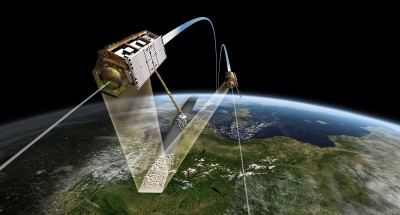
\includegraphics[scale=1]{media/main-body-chapter-intro/TandemX-wiki.jpg}
	\caption{TandemX.}\label{TandemX}
\end{figure}

\subsection{Subsección}

\begin{IEEEeqnarray}{rCl}
	\mathbf{\ddot{r}}_{SRP} & = & - \frac{p_{srp}\,C_R\,A_{srp}}{m} \, \frac{\mathbf{d}}{d} \label{eq:srp_def}
\end{IEEEeqnarray}

\begin{IEEEeqnarray}{rCl}
	A_c & = & r^2 + \norm{\vecbf{s - r}}^2\,\tau_{min}^2 + 2\,\left(\vecbf{s-r}\right)\cdot\vecbf{r}\,\tau_{min} \nonumber \\
	& = & r^2 + \left(s^2 + r^2 - 2\,\vecbf{r}\cdot\vecbf{s}\right)\,\tau_{min}^2 + 2\,\left(-r^2 + \vecbf{r}\cdot\vecbf{s} \right) \tau_{min} \nonumber \\
	& = & r^2\left(1 - 2\,\tau_{min}\right) + 2\,\vecbf{r}\cdot\vecbf{s}\,\tau_{min} + \frac{\left(r^2-\vecbf{r}\cdot\vecbf{s}\right)}{r^2+s^2-2\,\vecbf{r}\cdot\vecbf{s}} \\
	& = & r^2\left(1 - 2\,\tau_{min}\right) + 2\,\vecbf{r}\cdot\vecbf{s}\tau_{min} + \left(r^2 - \vecbf{r}\cdot\vecbf{s}\right)\,\tau_{min} \nonumber 
\end{IEEEeqnarray}

Donec egestas nisl purus, a dignissim neque venenatis tempor. Proin facilisis quam eget sem vulputate ultrices. Aliquam sed enim id enim tincidunt sodales eget in enim. Nulla eget finibus libero. Fusce non tristique elit, eget varius erat. Pellentesque malesuada, nulla non rhoncus condimentum, leo nisi sagittis lacus, vel lobortis eros est pretium neque. Nulla nunc justo, convallis sed nibh sit amet, bibendum consectetur lacus. \footnote{Nulla eget finibus libero. Fusce non tristique elit, eget varius erat. Pellentesque malesuada, nulla non rhoncus condimentum, leo nisi sagittis lacus, vel lobortis eros est pretium neque. Nulla nunc justo, convallis sed nibh sit amet, bibendum consectetur lacus.}\footnote{Nulla eget finibus libero. Fusce non tristique elit, eget varius erat. Pellentesque malesuada, nulla non rhoncus condimentum, leo nisi sagittis lacus, vel lobortis eros est pretium neque.}

Nullam sed porta risus. Nulla non metus quis quam porta laoreet. Donec egestas nisl purus, a dignissim neque venenatis tempor. Proin facilisis quam eget sem vulputate ultrices. Aliquam sed enim id enim tincidunt sodales eget in enim. Nulla eget finibus libero. Fusce non tristique elit, eget varius erat. Pellentesque malesuada, nulla non rhoncus condimentum, leo nisi sagittis lacus, vel lobortis eros est pretium neque. Nulla nunc justo, convallis sed nibh sit amet, bibendum consectetur lacus.\footnote{Nulla eget finibus libero. Fusce non tristique elit, eget varius erat. Pellentesque malesuada, nulla non rhoncus condimentum, leo nisi sagittis lacus, vel lobortis eros est pretium neque. Nulla nunc justo, convallis sed nibh sit amet, bibendum consectetur lacus.}


\begin{IEEEeqnarray}{rCl}
	\begin{bmatrix}
		\vecbf{r}(t_0) \\
		\vecbf{v}(t_0)
	\end{bmatrix}
	&=& 
	\begin{bmatrix}
		\SI{-7106.36}{\kilo\meter}  		  \\
		\SI{0}{\kilo\meter} 				  \\
		\SI{0}{\kilo\meter} 				  \\
		\SI{0}{\kilo\meter\per\second} 		  \\
		\SI{-1.04752}{\kilo\meter\per\second} \\
		\SI{7.45348}{\kilo\meter\per\second}
	\end{bmatrix} \quad \rightarrow \quad 
	\begin{bmatrix}
		a(t_0) \\
		e(t_0) \\
		i(t_0) \\
		\Omega(t_0) \\
		\omega(t_0) \\
		M(t_0)
	\end{bmatrix} = 
	\begin{bmatrix}
		\SI{7178.162}{\kilo\meter} \\
		\SI{0.01000}{} \\
		\SI{82}{\degree} \\
		\SI{180}{\degree} \\
		\SI{0}{\degree} \\
		\SI{0}{\degree} \\
	\end{bmatrix}
\end{IEEEeqnarray}

\section{How to cite references}

\begin{itemize}
	\item command: \textbackslash cite: \cite{alfriend_book}
	\item command: \textbackslash parencite: \parencite[10--100]{alfriend_book}
	\item command: \textbackslash textcite: \textcite[10--100]{alfriend_book}
	\item command: \textbackslash textcite con parentesis: (\textcite[10--100]{alfriend_book})
	\item command: \textbackslash citeauthor: \citeauthor{alfriend_book}
	\item command: \textbackslash textcite: \textcite[]{damico_thesis}
	\item command: \textbackslash parencite: \parencite[10--100]{jpl_de}
	\item command: \textbackslash textcite: \textcite[10--100]{jpl_de}
\end{itemize}